\section{Performance Evaluation}

Two platforms were for performance evaluation of our novel \textit{PackDrop} scheduler:
i) A tightly coupled \textit{Supercomputer} with $24$ (in $2$ separate NUMA nodes) PEs per node, using an Infiniband interconnection supported by Intel's Parallel Studio XE implementation of \texttt{MPI} (v2017.4).
ii) A smaller \textit{Cluster} with $4$ PEs per node, using a Gigabit Ethernet interconnection.
Details of both platforms are available on Table~\ref{tab:ptinfo}.

\begin{table}[ht]
    \centering
    \caption{Platform Information of each Node from Supercomputer and Cluster evaluations.}
	\begin{tabular}{c|c|c}
	Node Info.	 		& Supercomputer 		& Cluster \\ \hline
        CPUs	   			& $2\times12$ 			& $4$ \\
        Intel Xeon			& E5-2695v2 			& X3440\\
        CPU Freq.  			& $2.4$GHz   			& $2.53$GHz\\
        RAM        			& $64$GB			& $16$GB\\
        Network 			& Infiniband FDR 		& Gigabit Ethernet\\
        OS      			& RedHat Linux 6.4 		& Ubuntu 14.04\\
        \texttt{GCC}			& $5.3.1$			& $5.4.0$\\
        \texttt{Charm++} 		& $6.8.1$ 			& $6.8.1$\\
        \texttt{MPI}			& $3.1.0$			& -\\
        \texttt{GCC} Flags		& \texttt{-std=c++11 -O3} 	& \texttt{-std=c++11 -O3} \\
	\end{tabular}
    \label{tab:ptinfo}
\end{table}

Ahead we'll present the metrics used to compare our new global rescheduling strategy with \textit{Greedy}, \textit{Refine} and \textit{Distributed}.
Then, we'll discuss results obtained in both platforms descripted in Table~\ref{tab:ptinfo} and the scalability of our proposed solution.
All raw data of our results, as well as parsing scripts for analysis are publicly available\footnote{Available at: \texttt{https://github.com/eclufsc/\\packdrop-data-analysis}.}.

\subsubsection*{Metrics}

\textit{Application time} is one of the most relevant metrics to evaluate load balancers in \texttt{Charm++}.
Since migrations may induce high overhead and impact communication costs, a bad algorithm may finish fast, but increase imbalance, and thus, application time.

\textit{Load balancer decision time}, although not the most relevant for the application itself, the decision time is an indicator of its scalability.
Some centralized schedulers, such as \textit{Greedy}, work very well on local machines, with a reasonable data input.
However, when executing on distributed memory environments, the scalability of centralized strategies is limited.

\subsection{Evaluation on Cluster} \label{sec:cluster}

All experiments executed on cluster were compiled with \texttt{Charm++} using the \texttt{--with-production} option, combined with the specifications detailed on Table~\ref{tab:ptinfo}.
$32$ homogeneous compute nodes were used, with a total of $128$ PEs.
In addition to previously mentioned schedulers, \textit{Dummy} was added as the representative of a situation with no remap of tasks, it only aggregates the information a centralized strategy needs (its cost is the base for every centralized strategy).

\subsubsection{Evaluation with Synthetic Load} \label{sec:cluster:lbtest}

\textit{LB Test} experiments had a total of $18990$ \textit{tasks}, executed over $150$ iterations, performing load balance every $40$ iterations.
\textit{Task} loads vary from $30$ms to $9000$ms, which provides reasonable imbalance of load, causing global rescheduling to be useful in this case.
Ring, 2D mesh and 3D mesh communication topologies were used to provide different levels of migration impact and communication cost.

\begin{table}[t]
	\centering
    \caption{LB Test mean application time on the cluster execution.}
	\begin{tabular}{l | c  c  c}
    	Scheduler & Time (Ring) & Time (2D) & Time (3D) \\ \hline
        Distributed & $47.49298$s & $48.64839$s & $49.05481$s \\
        Greedy & $46.54101$s & $49.56052$s & $51.06850$s \\
        Dummy & $52.43016$s & $53.17254$s & $53.94068$s \\
        PackDrop & $46.81598$s & $47.37120$s & $47.97426$s \\
        Refine & $45.49095$s & $46.29277$s & $47.21924$s \\		
	\end{tabular}
    \label{tab:lbtest:apptime}
\end{table}

\begin{figure}
	\centering
    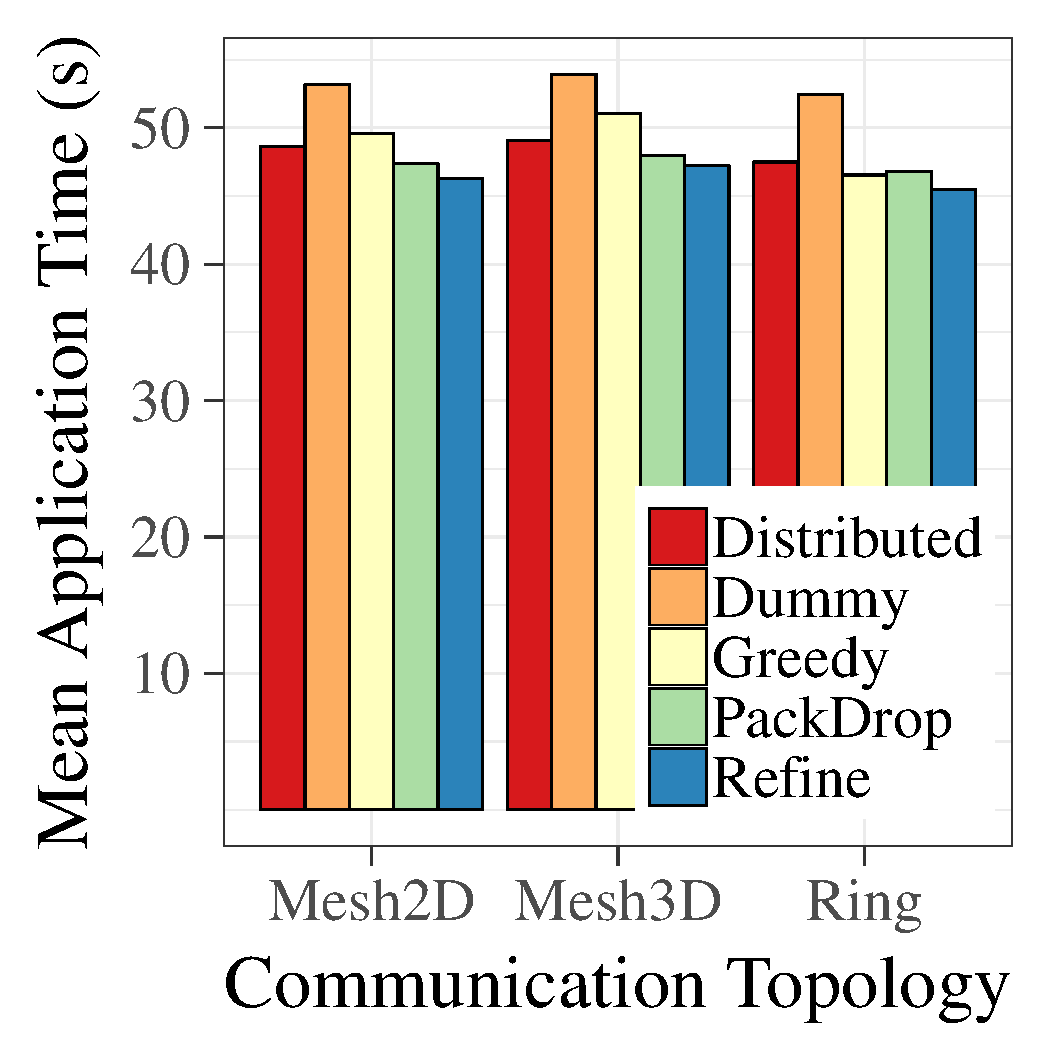
\includegraphics[width=\linewidth]{images/apptime_lbtest_g5k.pdf}
    \caption{LB Test cluster execution results.}
    \label{fig:eval:g5k:lbtest:apptime}
\end{figure}


Each configuration of the benchmark was executed $15$ times, with results depicted on Figure~\ref{fig:eval:g5k:lbtest:apptime} and Table~\ref{tab:lbtest:apptime}.
Results for \textit{Greedy} show how different communication topologies affect the scheduling performance.
Since \textit{Greedy} migrates many \textit{tasks}, the more they communicate, the more migrations impact the application time.

The increased in communication cost can be verified among all scheduling strategies, but in none as much as in \textit{Greedy}.
Our novel approach, \textit{PackDrop} has outperformed the other descentralized strategy, \textit{Distributed}, in the \textit{LB Test} case in this scale.
However, since the platform is not large enough to present all of the potential gains of decentralized strategies, \textit{Refine}, with a reduced migration count approach, still outperforms any other scheduler in this benchmark.
Nevertheless, this indicates a good scalability pontetial, specially in a cluster with high communication overhead, due to its Gigabit Ethernet connection.

\subsubsection{Evaluation with Molecular Dynamics} \label{sec:cluster:md}

\textit{LeanMD} experiments generated a $9\times9\times9$ space, with a total of $27702$ \textit{tasks}.
Each execution ran $500$ iterations, with a first rescheduling step at the $10$th iteration. 
Rescheduling periods (RP) of every $30$ (short) and every $60$ (long) iterations were used, providing different impacts of rescheduling on the application.
\textit{Greedy} and \textit{Dummy} were excluded from this evaluation due to their high cost in an application such as \textit{LeanMD}. 

\begin{table}[!ht]
	\centering
	\caption{LeanMD mean application time on the cluster execution.}	
	\begin{tabular}{l|c c c}
	Scheduler & Time (Short RP) & Time (Long RP) & Mean LB Time \\ \hline
	Distributed & $69.35606$s & $68.36055$s & $167.0444$ms \\ 
	PackDrop & $55.98428$s & $55.51554$s & $143.1028$ms \\ 
	Refine & $59.35696$s & $55.89895$s & $539.8364$ms \\ 
	\end{tabular}
	\label{tab:eval:g5k:leanmd:time} 
\end{table}

\begin{figure}[!ht]
	\centering
    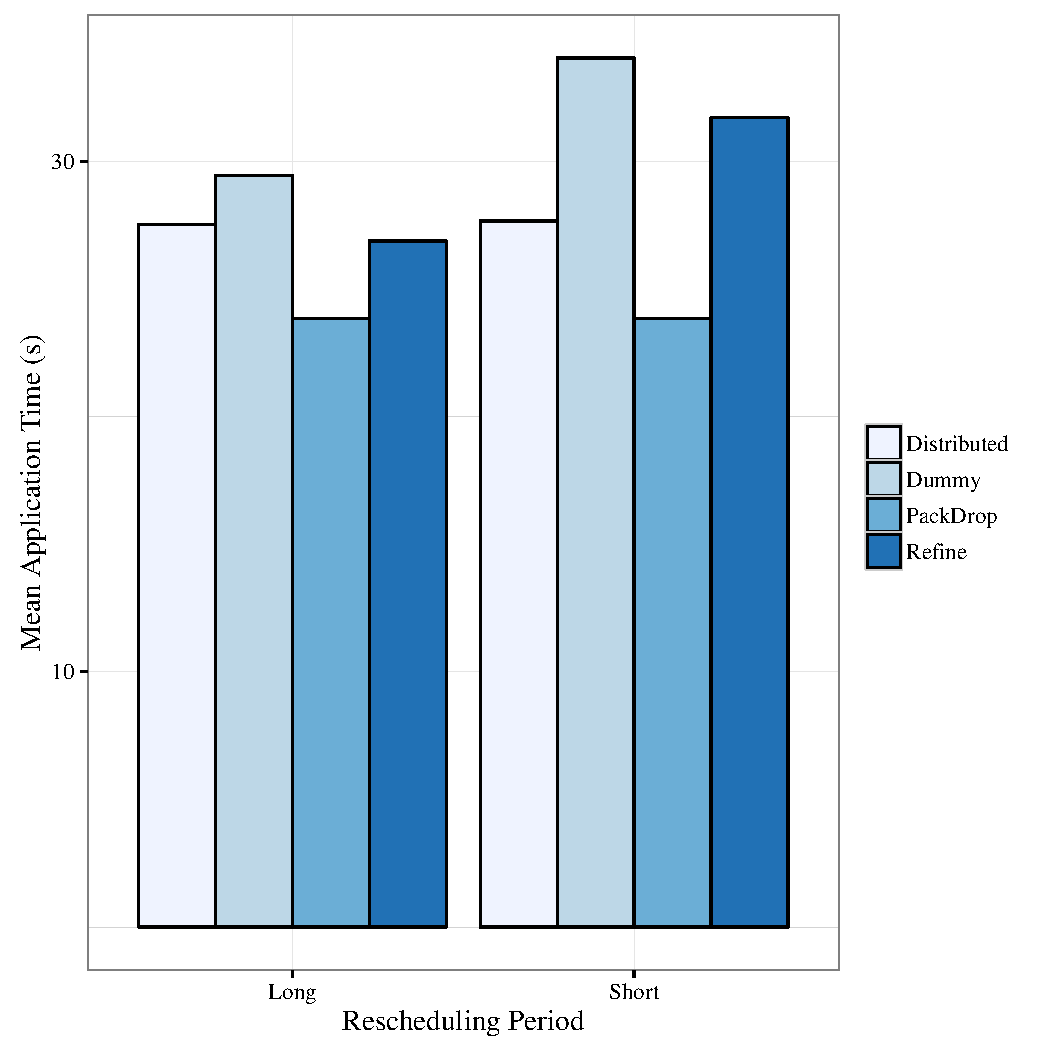
\includegraphics[width=0.43\textwidth]{images/apptime_leanmd_g5k.pdf}
	\caption{LeanMD cluster execution results.}
    \label{fig:eval:g5k:leanmd:time}
\end{figure}

\begin{figure}[!t]
	\centering
    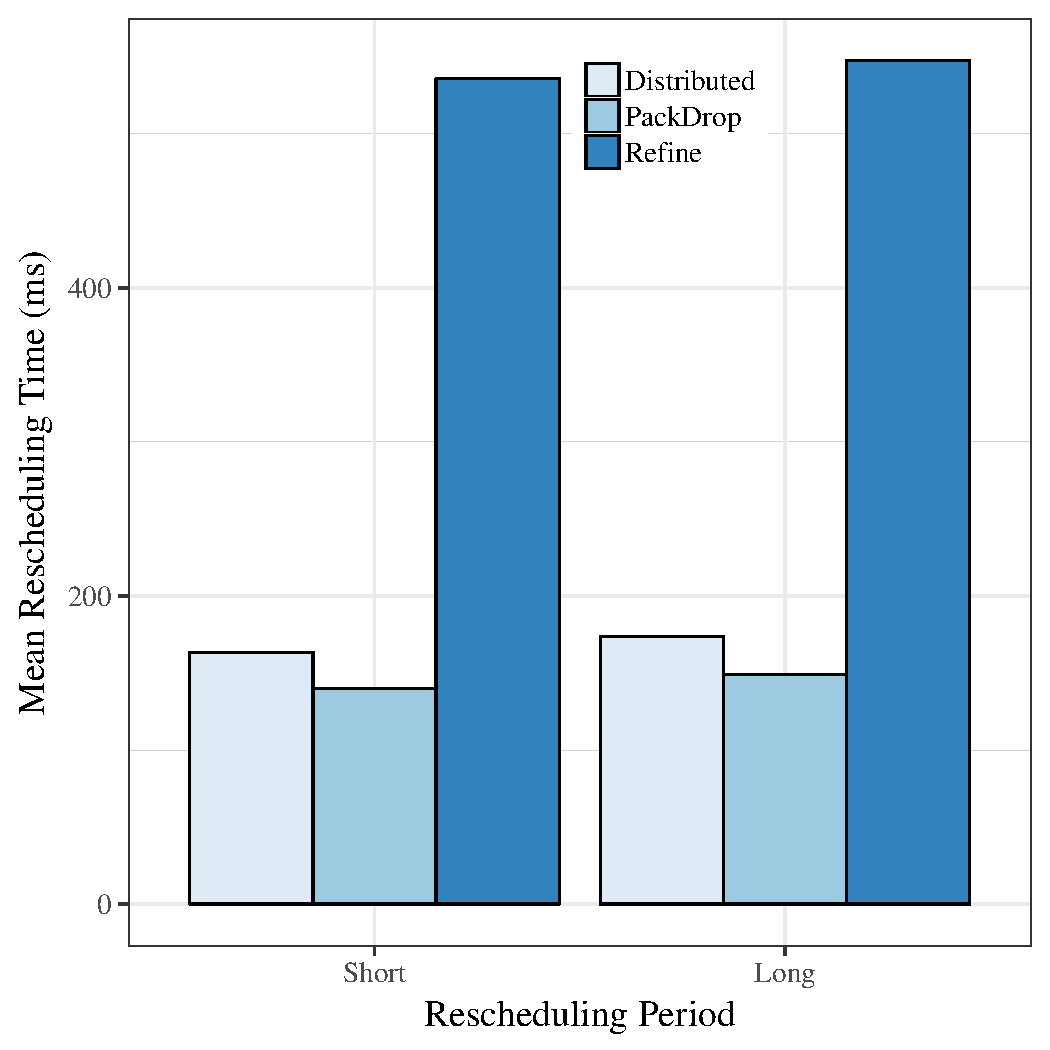
\includegraphics[width=0.43\textwidth]{images/schedtime_leanmd_g5k.pdf}
	\caption{LeanMD cluster execution results.}
    \label{fig:eval:g5k:leanmd:schedtime}
\end{figure}

Each configuration of LeanMD was executed $10$ times, making a total of $5000$ steps per configuration and are depicted in Table~\ref{tab:eval:g5k:leanmd:time} and in Figures~\ref{fig:eval:g5k:leanmd:time},~\ref{fig:eval:g5k:leanmd:schedtime}.
Observed application times presented a standard deviation from the mean lower than $2\%$ for all results presented.

Results show a better overall performance of \textit{PackDrop}, outperforming both compared strategies in the two scenarios chosen.
Since our strategy migrates groups of tasks, it improves locality of tasks after migration, outperforming \textit{Distributed} due to this.

Figure~\ref{fig:eval:g5k:leanmd:schedtime} shows the time taken by the periodical rescheduling (LB), task migration and the first iteration after the LB call.
It shows the increased cost of \textit{Refine}, which is due to both information agregation costs and dealing with the high amounts of application data in a centralized fashion.
\textit{PackDrop} displays its effectiviness in rescheduling time, outperforming both compared strategies, and resulting in an overall better application time. 

\subsection{Evaluation on Supercomputer} \label{sec:sdumont}

All experiments executed on supercomputer were compiled with \texttt{Charm++} using the \texttt{--with-production} option, combined with the specifications detailed on Table~\ref{tab:ptinfo}.
Different numbers of homogeneous $2\times 12$ PEs compute nodes ($2$ NUMA-nodes with $12$ cores each) were used to evaluate our strategy's scalability.
We ranged from $16$ ($384$ PEs) to $32$ ($768$ PEs) unique nodes in our evaluation. 

\subsubsection{Evaluation with Molecular Dynamics} \label{sec:sdumont:md}

\textbf{LeanMD} experiments generated a $10\times15\times10$ space, with a total of $171$K \textit{tasks}.
Each execution ran $100$ iterations, with a first rescheduling step at the $9$th iteration. 
Rescheduling was performed every $30$ iterations and each configuration of LeanMD was executed $10$ times, making a total of $1000$ steps per configuration. 

\begin{figure}[!ht]
 \centering
 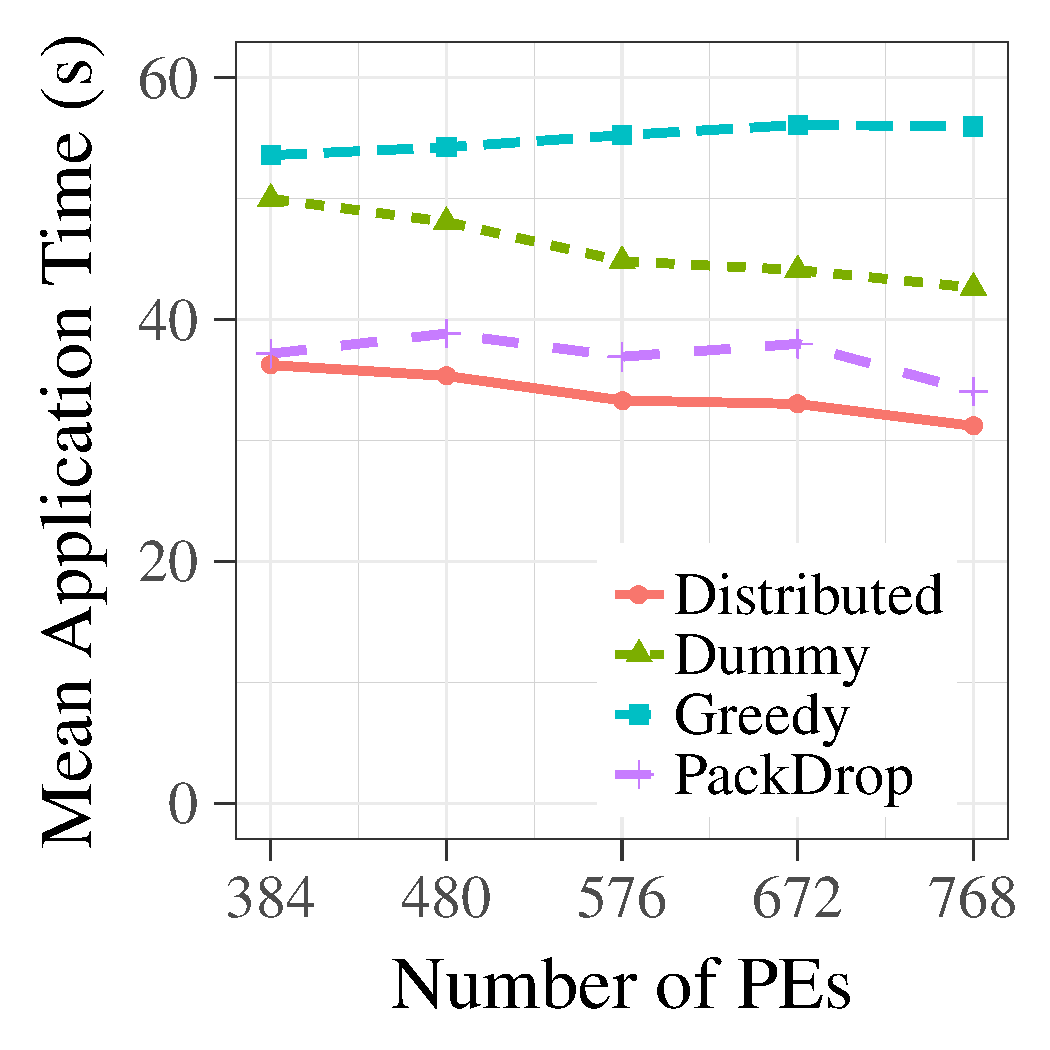
\includegraphics[width=0.9\linewidth]{images/apptime_leanmd_sdumont.pdf}
 \caption{LeanMD supercomputer AppTime execution results.}
 \label{fig:eval:sdumont:leanmd:apptime}
\end{figure}

%\begin{figure}[!ht]
% \centering
% 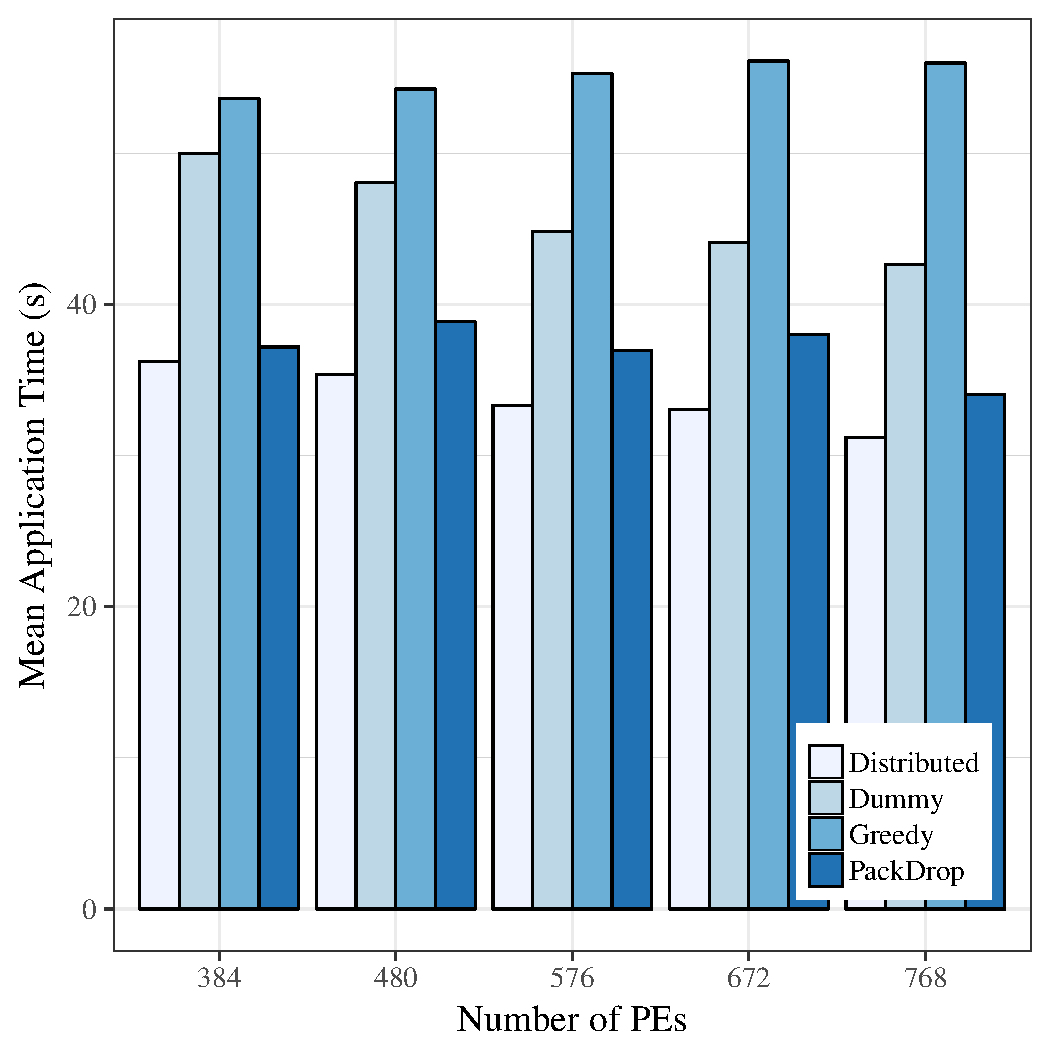
\includegraphics[width=0.9\linewidth]{images/apptime_leanmd_sdumont_bars.pdf}
% \caption{LeanMD supercomputer AppTime execution results.}
% \label{fig:eval:sdumont:leanmd:apptime:bars}
%\end{figure}

\begin{figure}
	\centering
	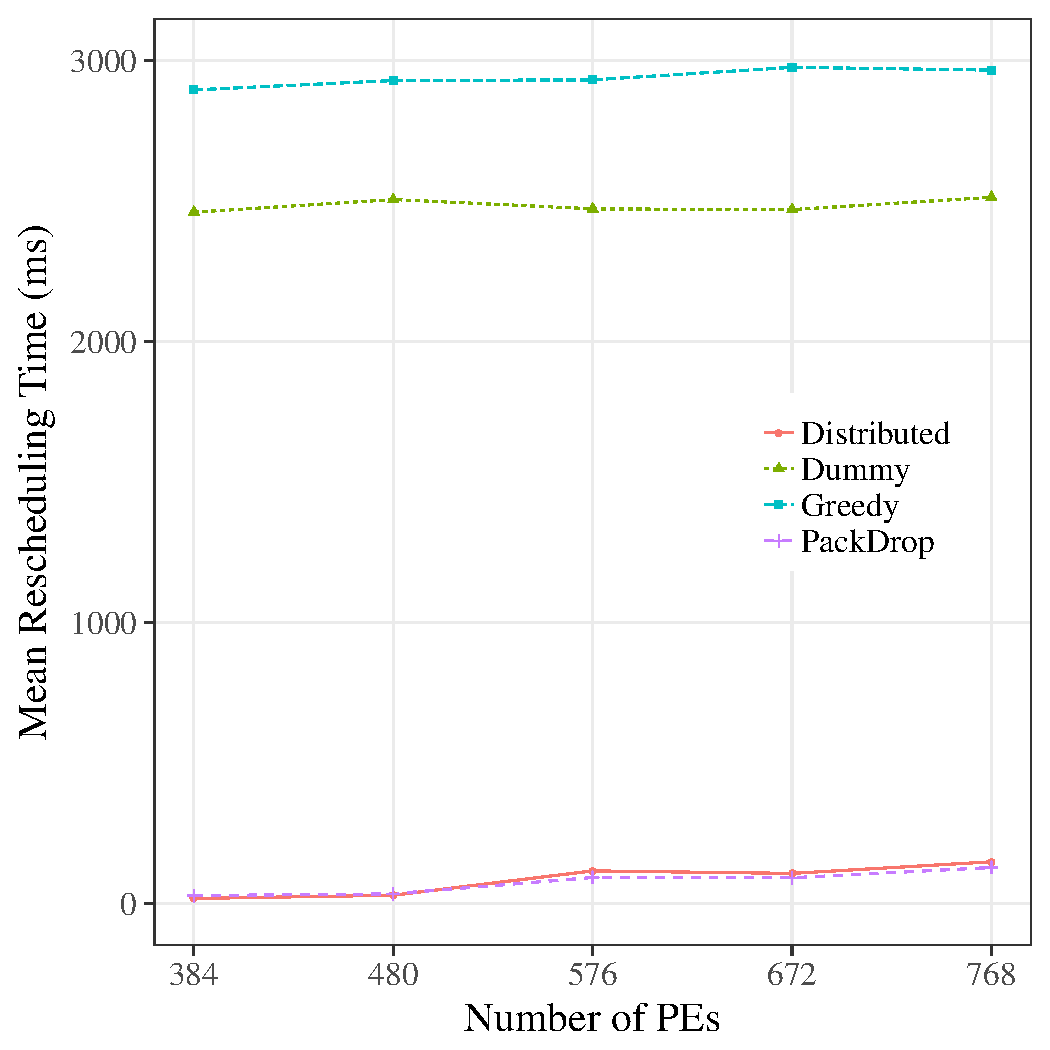
\includegraphics[width=0.9\linewidth]{images/schedtime_leanmd_sdumont.pdf}
	\caption{LeanMD supercomputer SchedTime execution results.}
	\label{fig:eval:sdumont:leanmd:schedtime}
\end{figure}

Results of mean application time are displayed in Figure~\ref{fig:eval:sdumont:leanmd:apptime} and mean rescheduling time in Figure~\ref{fig:eval:sdumont:leanmd:schedtime}.
\textit{Refine} was excluded from this evaluation since this LeanMD input presents more data than Refine is able to process in a reasonable time.

\textit{Distributed} benefits from this platform due to the Infiniband low latency communication, which reflects on improved total application times, as seen in Figure~\ref{fig:eval:sdumont:leanmd:apptime}.
Our novel approach, \textit{PackDrop}, followed it closely and we can see that its rescheduling time in larger systems outperforms \textit{Distributed}, displayed in Figure~\ref{fig:eval:sdumont:leanmd:schedtime}.

The rescheduling and application time results of LeanMD in this platform highlight the importance of using scalable approaches to load balancing, as well as using available parallism in execution environments.
This is specially visible in \textit{Greedy} results on Figure~\ref{fig:eval:g5k:lbtest:apptime}, where the application performance was decreased after the global rescheduling process.
Increased migration costs and higher \textit{hop} counts in communication, consequences of load balancing, heavily impacted LeanMD in this case.

\subsection{Performance Evaluation Overview} \label{eval:overview}

Most scientific applications today seek strong scaling, increasing their computational platforms to solve problems faster.
Our results show that, to achieve such an objective, an application must implement efficient load balancing strategies.
We present \textit{PackDrop} as a solution for scalable rescheduling of work in distributed memory systems.

Section~\ref{sec:cluster:lbtest} shows the efficiency of our strategy. 
Results highlight the importance of load balancing even in synthetic loads.
The \textit{LB Test} benchmark used has very low migration and communication overhead, and most of its work is done locally, which is optimal for rescheduling evaluation of raw computational workload.
Our strategy was only outperformed by \textit{Refine} in all test cases, which is expected, since the total load dealt with is considerably small ($\sim 19$K tasks) and migrations cheap, which benefits centralized schedulers.

Sections~\ref{sec:cluster:md}~and~\ref{sec:sdumont:md} display evaluation of a MD mini-app, LeanMD (better described in Section~\ref{sec:benchmarks}).
This represents ``a real world-like" scenario, in which applications may have dynamic communication patterns and high migration overhead.
Results presented here highlight the overhead of centralized rescheduling approaches when joined with large-scale applications ($171$K tasks) and big environments, which increases work and information aggregation costs, respectively.

\textit{Distributed} outperformed our approach in the Supercomputer platform, due to its more refined approach for load balancing and high-speed network interconnection.
However, the results show that \textit{PackDrop} and its locality friendly batching of tasks for migration guarantees better performance in the Cluster platform, which portrays a Gigabit Ethernet interconnection.
\textit{PackDrop} was able to efficiently scale applications among all observed platforms, and had a faster rescheduling time than \textit{Distributed} in most of the observed cases.
